\documentclass[letterpaper,10pt,conference]{ieeeconf}
\overrideIEEEmargins
\usepackage[T1]{fontenc}
\usepackage{amsmath,amsfonts}
\usepackage{algpseudocode}
\usepackage{algorithm}
\usepackage{array}
\usepackage[caption=false]{subfig}
\usepackage{tabularx}
\usepackage{colortbl}
\usepackage{textcomp}
\usepackage{stfloats}
\usepackage{multirow}
\usepackage{verbatim}
\usepackage{graphicx}
\usepackage{cite}
\usepackage{flushend}
\usepackage{diagbox}
\usepackage[dvipsnames]{xcolor}
\usepackage{threeparttable}
\usepackage{booktabs}
\usepackage{empheq}
\usepackage{makecell}
\usepackage{url}
\usepackage{soul}
\usepackage{tikz}
\let\labelindent\relax
\usepackage{enumitem}
\usepackage{gensymb}
\usepackage{amssymb}
\usepackage[colorlinks=true, linkcolor=black, citecolor=black, urlcolor=blue]{hyperref}
\urlstyle{same} % makes the URL use the normal text font (not typewriter)
\definecolor{redvw}{HTML}{F36B9C}
\definecolor{bluevw}{HTML}{1E88E5}
\definecolor{greenvw}{HTML}{005648}
\definecolor{navyblue}{RGB}{0, 83, 137}

\newcommand{\victor}[1]{{\color{navyblue}#1}}
\newcommand{\victornote}[1]{{\color{orange}#1}}
\newcommand{\rp}[1]{{\color{blue}#1}}

\newcommand{\Estar}{E_{\star}}
\newcommand{\dd}{\mathrm{d}}
\newcommand{\ind}{\mathbf{1}}



\title{\bfseries Hierarchical Energy-Work Control for Rotary-Pendulum Capture}
\author{}




\begin{document}
\maketitle
\thispagestyle{empty}
\pagestyle{empty}

\section{Introduction}
% Act--coast control trades enabled operation against continued task performance.
Act--coast control alternates bounded actuation with intervals of unforced motion. The controller applies a planned input while enabled and commands zero input during coast, allowing the plant to follow its natural dynamics. The aim is to reduce enabled time and the frequency of feedback decisions while meeting a prescribed task and respecting operating constraints. The controller must therefore determine both how to act and when feedback is needed again.

% The input and coast duration jointly determine the next feedback state.
Coast duration cannot be selected independently of the preceding input. Actuation determines the state at switch-off, while unforced evolution determines the state at the next feedback decision. A longer coast can reduce intervention but also permit motion toward a constraint or away from the target. Each input and timing choice must therefore be assessed through the complete intervening motion and the control required afterward.

% The research objective is controller synthesis and analysis on a chosen benchmark.
We seek a bi-level controller in which outer model predictive control (MPC) selects both shut-off and replanning times, while an inner problem optimizes the bounded input for those times. Figure~\ref{fig:act-coast-overview} illustrates the complete event, with model prediction for its two parts and a continuation estimate for motion beyond its endpoint. The aim is a construction algorithm, sufficient conditions for admissible evolution between decisions, and quantified task and resource performance. We examine the predictive-control ingredients in nominal simulation on a rotary-pendulum benchmark.

% The vector overview spans both columns and is placed at the page top.
\begin{figure*}[t]
\centering
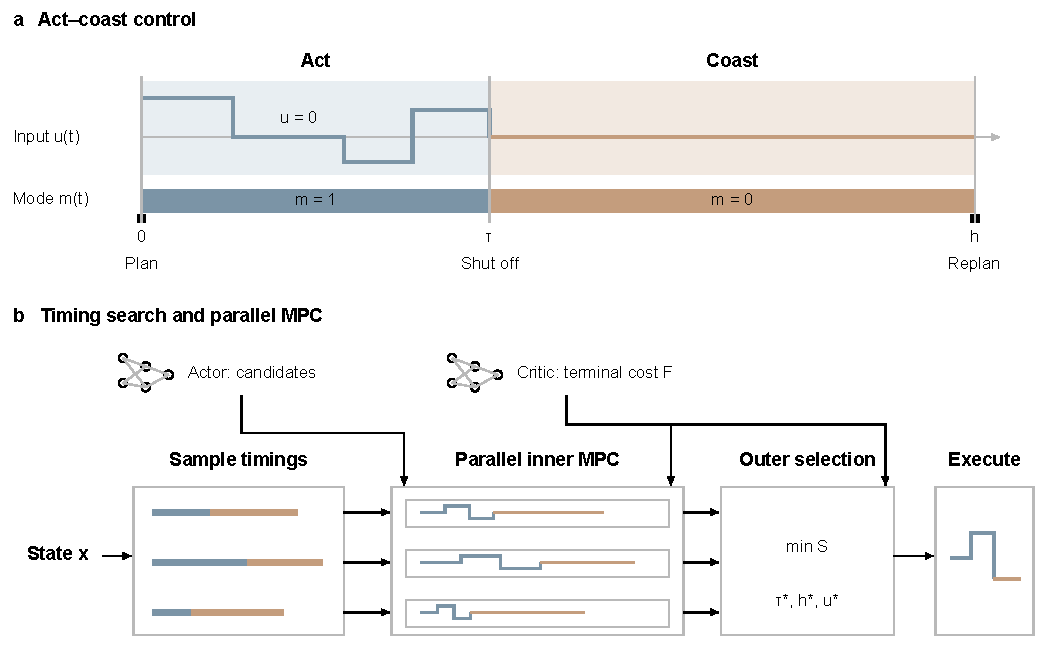
\includegraphics[width=\textwidth]{figures/act-coast-overview/figure-1-act-coast.pdf}
\caption{Act--coast concept and proposed controller construction.
(a) Time starts at the current decision. Input $u(t)$ executes planned commands until shut-off at $\tau$, then remains zero until replanning at $h$. Mode $m(t)$ is one during enabled operation and zero during coast, so an enabled zero command remains distinct from coast. Squares mark feedback decisions.
(b) At observed state $x$, outer MPC samples timing pairs $(\tau,h)$. One conditional inner MPC problem per pair optimizes the bounded input sequence; these problems are solved in parallel. The actor supplies candidates, and the critic-based terminal cost $F$ estimates actor continuation at each predicted replanning state. Thus $F$ influences both input optimization and the minimized event scores $S$ used for outer timing selection. The two critic arrows show this shared dependence; each event score includes its terminal cost once. Stars identify the selected times and input sequence $u^\star$. Miniature timing bars and input traces are schematic. The complete timing-conditioned construction remains to be evaluated.}
\label{fig:act-coast-overview}
\end{figure*}


\section{Problem Formulation}
% State and input constraints apply to both forced and unforced motion.
Consider the nominal nonlinear plant $\dot x=f(x,u)$ in continuous time $t$, with physical state $x$ and commanded input $u$. The known dynamics $f$ admit unique trajectories for admissible planned inputs, whose values belong to a prescribed bounded set $\mathcal U$ containing zero. The full state is observed at scheduled decision times, starting from $x(0)\in\mathcal X_0\subseteq\mathcal X$, where $\mathcal X_0$ and $\mathcal X$ are the prescribed initial-state and operating sets. The constraints $x(t)\in\mathcal X$ and $u(t)\in\mathcal U$ apply throughout executed motion, including coast under $f(x,0)$.

% Each event executes an enabled input segment followed by zero-input coast.
Each decision selects an enabled input segment and the coast that follows it. At time $t_j$, with event index $j=0,1,\ldots$ and $t_0=0$, choose event duration $h_j$, enabled duration $\tau_j$, and planned input $v_j(s)\in\mathcal U$ for elapsed time $s\in[0,\tau_j)$, giving
\begin{equation}
\begin{aligned}
 t_{j+1}&=t_j+h_j,\\
 u(t)&=\begin{cases}
 v_j(t-t_j),&t_j\le t<t_j+\tau_j,\\
 0,&t_j+\tau_j\le t<t_{j+1}.
 \end{cases}.
\end{aligned}
\label{eq:act-coast}
\end{equation}
The first branch executes the planned actuation, and the second allows unforced evolution until feedback resumes at $t_{j+1}$. Prescribed bounds $0<h_{\min}\le h_j\le h_{\max}<\infty$ prevent accumulation of decisions in finite time, while $0<\tau_j<h_j$ requires both intervals to be nonempty. Define the mode indicator $m(t)$ as one while enabled and zero during coast, so an enabled zero command remains distinct from disabled operation.

% Task success requires uninterrupted target residence within the assessment horizon.
Task completion requires reaching a prescribed target neighborhood and remaining there for a prescribed duration. For a chosen task-error map $e$, Euclidean norm $\|\cdot\|$, and tolerance $\varepsilon>0$, define $\mathcal G=\{x\in\mathcal X:\|e(x)\|\le\varepsilon\}$. Within assessment duration $T>0$, success requires an entry time $t_g\in[0,T-T_{\mathrm{hold}}]$ such that $x(t)\in\mathcal G$ throughout $[t_g,t_g+T_{\mathrm{hold}}]$, where $0<T_{\mathrm{hold}}\le T$ is the required hold duration. This uninterrupted residence distinguishes continued regulation from a single target visit, while admissibility remains required throughout the assessment.

% Enabled duration and decision count give switch-off and feedback timing explicit costs.
The performance objective accounts for enabled time and new decisions alongside task error and input effort. For a chosen nonnegative running cost $\ell(x,u)$ and positive design weights $c_{\mathrm{on}},c_{\mathrm{dec}}$, define
\begin{equation}
\begin{aligned}
 T_{\mathrm{on}}&=\int_0^T m(t)\,\dd t,\qquad
 n(T)=\#\{j:0\le t_j<T\},\\
 J_T&=\int_0^T\ell(x(t),u(t))\,\dd t\\
 &\quad+c_{\mathrm{on}}T_{\mathrm{on}}+c_{\mathrm{dec}}n(T).
\end{aligned}
\label{eq:act-coast-cost}
\end{equation}
Here $T_{\mathrm{on}}$ is total enabled duration, $\#$ denotes counting, and $n(T)$ counts decisions including the initial one. The running cost expresses task and input preferences, while the two charges make switch-off consequential even at zero input and attach a cost to repeated decisions. Task completion and path admissibility remain requirements on this comparison.

% Evaluation separates task quality, resource use, and analytical admissibility.
The synthesis problem is to construct a state-dependent rule for Eq.~\eqref{eq:act-coast} that meets these requirements with low cost~\eqref{eq:act-coast-cost} on its feasible initial-state domain. Primary measures are task success, the earliest hold-completion time $t_g+T_{\mathrm{hold}}$ satisfying the residence condition, constraint violations, enabled fraction $T_{\mathrm{on}}/T$, and decision rate $n(T)/T$. Input effort $\int_0^T\|u(t)\|^2\,\dd t$ and task-error root mean square $(T^{-1}\int_0^T\|e(x(t))\|^2\,\dd t)^{1/2}$ quantify the accompanying control performance. Comparisons retain failed runs and use common dynamics, initial conditions, limits, target, and duration for act--coast control and periodic feedback with continuous enablement. An admissibility certificate must establish constraint satisfaction between decisions, beyond checks at finitely many prediction nodes.

\section{Method}
% The benchmark and learned predictive controller supply the inner-control ingredients.
The methods develop predictive-control ingredients for the act--coast design. Section~\ref{sec:dynamics} introduces the benchmark dynamics and energy representation, and Section~\ref{sec:contorller} constructs a teacher that supplies learning references. Section~\ref{sec:learning} learns a stationary policy and continuation value from these references and further interaction. Section~\ref{sec:mpc-rl} combines them with constrained nonlinear MPC, using a fixed prediction horizon and replanning after each held command as an inner-control baseline. Section~\ref{sec:bilevel} formulates outer MPC timing selection around conditional input optimization.

\subsection{Rotary-pendulum dynamics and energy representation}
\label{sec:dynamics}
% Benchmark coordinates retain the physical phase required for prediction.
Our chosen benchmark (Fig.~\ref{fig:rotary-pendulum-geometry}) is a rotary pendulum whose passive rod swings in an arm-attached vertical plane perpendicular to the motor-driven arm. The unwrapped arm angle $\theta\in\mathbb R$ is measured from a fixed horizontal reference, and the pendulum angle $\alpha\in[-\pi,\pi)$ is measured from downward. Signed angular speeds $\omega=\dot\theta$ and $\nu=\dot\alpha$, defined before angular wrapping, give physical state $x=(\theta,\alpha,\omega,\nu)^{\mathsf T}$ and coordinates $q=(\theta,\alpha)^{\mathsf T}$. For uniform rigid rods with ideal joints and zero damping, kinetic and potential energies are $K=\tfrac12\dot q^{\mathsf T}M(\alpha)\dot q$ and $V=G(1-\cos\alpha)$, where $M$ is the coupled inertia matrix and $G$ is pendulum mass times gravity times its center-of-mass distance from the hinge. The Lagrangian $\mathcal L=K-V$ retains mixed kinetic energy because arm motion carries the pendulum hinge.

% The benchmark specializes the generic limits and orientation-holding criterion.
Motor torque and arm travel satisfy $|u|\le U$ and $|\theta|<\theta_{\max}$, where $U,\theta_{\max}>0$ are prescribed bounds and positive torque increases $\theta$. Numerical commands are held over a fixed duration $\Delta>0$. Define the upright error $\beta=\operatorname{wrap}(\alpha-\pi)$, where $\operatorname{wrap}$ selects the equivalent angle in $[-\pi,\pi)$, and use $e(x)=\beta$ with prescribed angular tolerance $\varepsilon=\varepsilon_\alpha>0$. This target tests orientation, while ideal upright rest additionally requires $\omega=\nu=0$.

% The benchmark schematic occupies one column with symbolic constraints.
\begin{figure}[t]
\centering
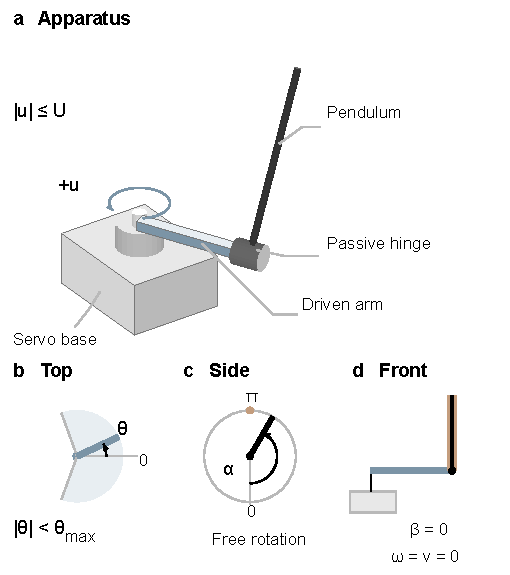
\includegraphics[width=\columnwidth]{figures/rotary-pendulum-geometry/figure-2-rotary-pendulum.pdf}
\caption{Rotary-pendulum apparatus and benchmark requirements.
(a) The servo drives the blue horizontal arm; its end hinge supports a passive rod with rotation axis parallel to the arm.
(b) Top view: the unwrapped arm angle $\theta$ is measured from a fixed reference, and positive shaft torque $u$ increases $\theta$. Prescribed hard design limits are $|\theta|<\theta_{\max}$ and $|u|\le U$, with $\theta_{\max},U>0$.
(c) Side view: the rod rotates freely in the arm-normal vertical plane; $\alpha=0$ is downward and $\alpha=\pi$ is upright.
(d) Front view: ideal upright rest has $\beta=\operatorname{wrap}(\alpha-\pi)=0$ and $\omega=\nu=0$, where $\omega=\dot\theta$ and $\nu=\dot\alpha$ are angular speeds, with wrapping to $[-\pi,\pi)$. The apparatus is schematic. Exact design limits and the ideal rest reference are shown; numerical penalties and finite-tolerance assessment are specified separately in the text.}
\label{fig:rotary-pendulum-geometry}
\end{figure}


% The forced Euler--Lagrange relation supplies the physical prediction model.
Differentiating $\mathcal L$ relates joint torques to accelerations through $\frac{\dd}{\dd t}(\partial\mathcal L/\partial\dot q)-\partial\mathcal L/\partial q=(u,0)^{\mathsf T}$. With torque applied only to the arm, this gives
\begin{equation}
\begin{aligned}
 M(\alpha)&=\begin{bmatrix}A(\alpha)&C(\alpha)\\C(\alpha)&J\end{bmatrix},\\
 M(\alpha)\ddot q&+
 \begin{bmatrix}
 A'\omega\nu+C'\nu^2\\
 -\tfrac12 A'\omega^2+G\sin\alpha
 \end{bmatrix}
 =\begin{bmatrix}u\\0\end{bmatrix}.
\end{aligned}
\label{eq:dynamics}
\end{equation}
Here $A=J_0+J\sin^2\alpha$, $C=B\cos\alpha$, and primes denote differentiation with respect to $\alpha$; the fixed coefficients $J_0,J,B$ are the baseline arm-axis inertia including the carried pendulum, pendulum hinge inertia, and inertial coupling coefficient, respectively, computed from link geometry and masses. The off-diagonal entries couple the accelerations, while the remaining terms describe velocity-dependent inertial torques and gravity. Solving for the accelerations and adjoining $\dot\theta=\omega$, $\dot\alpha=\nu$ defines the physical-state dynamics $\dot x=f(x,u)$, whose integration predicts motion under a proposed torque.

% The energy partition distinguishes motion from the elevation needed at upright rest.
Upright rest requires mechanical energy to become gravitational potential rather than remain kinetic motion. Separate the arm-body kinetic energy $K_a=\tfrac12 I_a\omega^2$, where $I_a$ is the arm's own motor-axis inertia, from the pendulum-body kinetic energy $K_p=K-K_a$, which includes hinge motion and coupling. These define the energy map $H$, energy representation $z$, total energy $E$, and upright-rest energy $\Estar$ by
\begin{equation}
\begin{aligned}
 z=H(x)&=(K_a,K_p,V)^{\mathsf T},\\
 E&=K_a+K_p+V,\qquad \Estar=2G.
\end{aligned}
\label{eq:encoder}
\end{equation}
Since $K_a+K_p=E-V$, bringing both $E$ and $V$ toward $\Estar$ removes the remaining kinetic energy and motivates the teacher's energy feedback.

% Physical phase determines the direction of energy exchange.
Energy feedback specifies a desired correction, while physical phase determines its realization. Differentiating $E=K+V$ along Eq.~\eqref{eq:dynamics} cancels internal energy exchange, and differentiating $V$ gives
\begin{equation}
 \dot E=u\omega,\qquad \dot V=G\sin\alpha\,\nu.
\label{eq:powers}
\end{equation}
Motor power changes total energy, while pendulum orientation and signed velocity determine whether potential energy rises or falls. States with opposite $\alpha$ and otherwise identical coordinates have the same $z$ but opposite $\dot V$ when $\sin\alpha\,\nu\ne0$. The teacher therefore uses the full physical state to predict energy transfer.

\subsection{Mechanical teacher and demonstration trajectories}
\label{sec:contorller}
% Bounded work feedback guides the search for a nominal torque.
The energy-based heuristic~\cite{astrom2000} requests bounded work from the difference between current and upright-rest energy. For a chosen gain $\kappa>0$, work bound $\bar w>0$, and action duration $\Delta>0$, define requested work $w$ and work $\mathcal W(x,u)$ delivered from initial state $x$ by a constant torque as
\begin{equation}
\begin{aligned}
 w&=\operatorname{clip}\bigl(\kappa(\Estar-E),-\bar w,\bar w\bigr),\\
 \mathcal W(x,u)&=\int_0^\Delta u\omega(s)\,\dd s
 =u[\theta(\Delta)-\theta(0)].
\end{aligned}
\label{eq:workpolicy}
\end{equation}
Here $\operatorname{clip}$ restricts the request to the stated bounds, and $\theta(s),\omega(s)$ are the predicted arm angle and speed at elapsed time $s$, so work follows from the arm displacement under constant torque. Positive $w$ requests energy addition and negative $w$ energy removal, defining a total-energy budget whose attainable distribution depends on physical phase. Within $|u|\le U$, work matching supplies additional trial torques that compete with the sampled torques under potential-energy and arm-excursion penalties.

% The augmented teacher provides references for stationary policy and value learning.
The student needs reference trajectories containing both swing-up and continued upright control. The demonstration teacher therefore combines the nominal energy action with local linear balancing feedback near upright and predictive braking of outward arm motion. Trajectories satisfying the prescribed upright-holding and arm-bound conditions provide state--action examples and approximate return labels for initialization and remain available through demonstration replay. The student uses these references and its own transitions to learn a stationary torque policy and continuation-value estimates.

% Local energy authority explains the state dependence of a work request.
The same torque can affect total energy and pendulum swing energy differently. Define the relative swing energy $E_h=\tfrac12J\nu^2+V$, which excludes motion carried by the arm, and the instantaneous power sensitivities $s_E=\partial\dot E/\partial u$ and $s_h=\partial\dot E_h/\partial u$ at fixed state. The inertia relation gives
\begin{equation}
\begin{aligned}
 s_E&=\omega, & s_h&=-\frac{JC\nu}{AJ-C^2},\\
 c_E&=(E-\Estar)s_E, & c_h&=(E_h-\Estar)s_h.
\end{aligned}
\label{eq:energy-authority}
\end{equation}
Here $A,C,J$ are the inertia entries in Eq.~\eqref{eq:dynamics}; $c_E$ and $c_h$ are the torque coefficients in the derivatives of the respective half-squared energy errors, so equal nonzero signs admit a common reducing torque sign, while opposite signs imply competing input contributions. Figure~\ref{fig:energy-control} connects this local diagnostic to the teacher's energy request; natural energy exchange remains in the complete swing-energy rate, so these signs alone neither establish task progress nor select event times.

% Model-derived energy geometry and input authority at single-column width.
\begin{figure}[t]
\centering
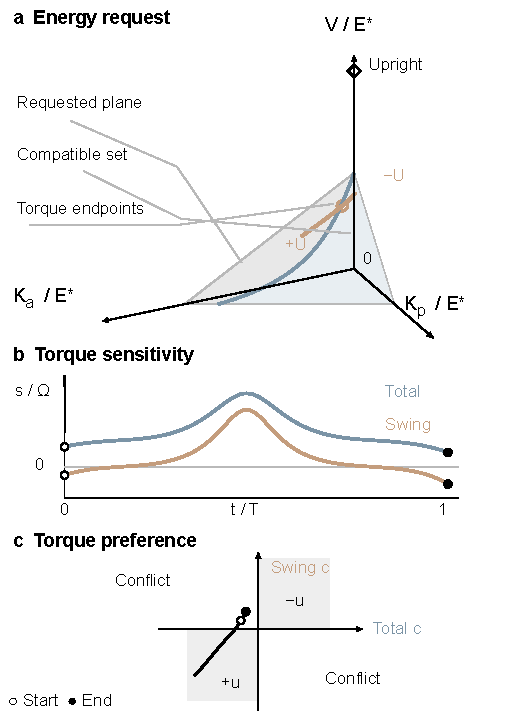
\includegraphics[width=\columnwidth]{figures/energy-control/figure-3-energy-control.pdf}
\caption{Energy requests and state-dependent input directions.
(a) The requested-work plane satisfies $K_a+K_p+V=E+w$, where $E$ is the initial total energy and $w$ is the teacher's requested work. Its blue subset contains mechanically compatible energy distributions, obtained by minimizing pendulum-body kinetic energy over the hinge speed at each arm energy and potential. The orange curve contains endpoints under constant torques in $[-U,U]$ over one fixed duration; the open circle marks work matching. Neither set is a complete bounded-input reachable set. Axes use upright-rest energy $\Estar$, denoted $E^*$ in the artwork; the diamond is $(0,0,\Estar)$.
(b) Blue total-energy and orange relative-swing sensitivities from Eq.~\eqref{eq:energy-authority}, divided by the model's downward small-motion frequency $\Omega>0$, along a constructed zero-input segment. Time is divided by $T=2\pi/\Omega$.
(c) The same segment in $(c_E,c_h)/(\Estar\Omega)$ coordinates. Gray quadrants admit the indicated common torque sign for reducing both input contributions; the other quadrants indicate conflict, and zero axes indicate zero corresponding direct authority. Open and filled markers identify segment start and end. Natural transfer remains in the complete swing-energy rate; these diagnostics do not certify coast duration, arm admissibility, or closed-loop performance.}
\label{fig:energy-control}
\end{figure}


\subsection{Stationary policy and continuation-value learning}
\label{sec:learning}
% A physical-state observation preserves the phase information needed for torque selection.
The student learns a torque rule that retains the physical phase needed for swing-up and upright holding. Its observation is $o=\operatorname{normalize}(\theta,\sin\alpha,\cos\alpha,\omega,\nu)$, where $\operatorname{normalize}$ applies fixed componentwise scaling and the sine--cosine pair represents pendulum orientation continuously across angular wrapping. An actor $\pi$ maps this observation to normalized torque $a=\pi(o)\in[-1,1]$, giving physical torque $u=Ua$. This policy is stationary because its action depends on the current physical observation. Fitting the teacher's actions initializes the actor, while value learning evaluates the motion that follows its choices.

% A continuing return assigns value to both swing-up and sustained upright motion.
Useful torque must contribute both to reaching upright and to remaining there with low speeds. Let $r_k$ be the negative accumulated cost over command interval $k$, using fixed positive weights to favor upright low-speed motion and penalize squared normalized torque and quadratic arm-centering and near-boundary terms. The additional penalty $|E_h/\Estar-1|$ supplies a swing-energy target away from upright; the teacher's mechanical energy $E$ also includes arm motion and coupling. For initial observation $o_0=o$, initial action $a_0=a$, and chosen per-command discount $0<\gamma<1$, the ideal policy action value is
\begin{equation}
 Q^\pi(o,a)=\mathbb E_\pi\!\left[
 \sum_{k=0}^{\infty}\gamma^k r_k
 \;\middle|\;o_0=o,\ a_0=a
 \right].
\label{eq:policy-value}
\end{equation}
Here $k$ indexes command intervals and $\mathbb E_\pi$ averages subsequent trajectories under $\pi$, so discounting gives greater weight to near-term rewards while the continuing sum values sustained holding.

% Twin critics extend teacher-return estimates through bootstrapped student transitions.
Approximate discounted teacher returns initialize two critics $Q_1,Q_2$ that estimate $Q^\pi$, and mixed replay combines retained demonstrations with the student's new transitions. We use Twin Delayed Deep Deterministic Policy Gradient (TD3)~\cite{fujimoto2018}, with slowly updated target copies $\bar\pi,\bar Q_1,\bar Q_2$ to limit changes in the continuation estimate used for training. For a sampled transition $(o,a,r,o')$, with reward $r$, next observation $o'$, and bounded smoothing noise $\eta$, the perturbed target action $\widetilde a$ and value target $y$ are
\begin{equation}
\begin{aligned}
 \widetilde a&=\operatorname{clip}\bigl(\bar\pi(o')+\eta,-1,1\bigr),\\
 y&=r+\gamma\min_{j\in\{1,2\}}\bar Q_j(o',\widetilde a).
\end{aligned}
\label{eq:td-target}
\end{equation}
Clipping enforces the normalized torque range, both critics fit $y$ by squared-error regression, and the lower next-value estimate tempers optimistic bootstrapping. Learning continues after reaching upright, and sampling cutoffs retain the physical next observation and its continuation target.

% Retained imitation guides actor improvement while new experience refines the value estimates.
The actor improves its choices while retaining the teacher as a reference. Averaging over mixed replay distribution $\mathcal B$ and demonstration distribution $\mathcal D$, it minimizes the actor loss
\begin{equation}
\begin{aligned}
 L_\pi={}&-\mathbb E_{\mathcal B}Q_1(o,\pi(o))\\
 &+\lambda\mathbb E_{\mathcal D}
 \left[\bigl(\pi(o)-a_{\rm teach}\bigr)^2\right].
\end{aligned}
\label{eq:actor-loss}
\end{equation}
Here $a_{\rm teach}$ is the normalized teacher action and $\lambda>0$ is the chosen imitation weight, so the negative critic term favors larger estimated return while the squared error penalizes departure from demonstrated actions. Actor updates occur less frequently than critic updates, allowing value estimates to adjust between policy changes. The trained actor and critics are then frozen for predictive control, supplying candidate continuations and estimates of their future return.

\subsection{Nonlinear predictive control with learned continuation}
\label{sec:mpc-rl}
% The frozen critics assign a continuation cost to each predicted endpoint.
Finite-horizon control must judge both the predicted motion and the continuation beyond its endpoint. With the trained actor $\pi$ and critics $Q_1,Q_2$ held fixed, define the terminal cost at physical state $x$ by
\begin{equation}
 F(x)=-\min_{j\in\{1,2\}}Q_j\bigl(o(x),\pi(o(x))\bigr).
\label{eq:terminal-value}
\end{equation}
Here $o(x)$ is the physical observation defined in Section~\ref{sec:learning}, and negating the lower reward estimate assigns a larger cost to less favorable continuation. Thus $F$ estimates the cost of following the learned policy under its training reward.

% Nonlinear prediction combines quadratic motion costs with the learned endpoint score.
At each update, MPC balances predicted state error and control effort against this continuation score. For a fixed horizon length $N$ and observed state $x$, it predicts states $x_i$ under normalized commands $\mathbf a=(a_0,\ldots,a_{N-1})$, using the map $\Phi_\Delta$ obtained by numerically integrating $\dot x=f(x,Ua_i)$ over the fixed command duration $\Delta$. With predictive state error $\xi_i=\xi(x_i)$, $\xi(x)=(\theta,\beta,\omega,\nu)^{\mathsf T}$, a fixed positive diagonal state weight $W$, and a fixed positive scalar input weight $R$ inherited from the discrete linear-quadratic design, the prediction problem is
\begin{equation}
\begin{aligned}
 \min_{\mathbf a}\quad&
 \sum_{i=0}^{N-1}\left(\xi_i^{\mathsf T}W\xi_i+Ra_i^2\right)+F(x_N),\\
 \text{subject to}\quad&x_0=x,\qquad x_{i+1}=\Phi_\Delta(x_i,a_i),\\
 &|a_i|\le1,\qquad |\theta(t)|<\theta_{\max},\quad t\in\mathcal T.
\end{aligned}
\label{eq:mpc-problem}
\end{equation}
Here $i=0,\ldots,N-1$, $x_N$ is the terminal predicted state, and $\mathcal T$ is the prescribed set of elapsed forecast integration times at which the predicted arm angle $\theta(t)$ is checked against $\theta_{\max}$. The undiscounted quadratic sum penalizes arm displacement, upright error $\beta$, angular speeds, and torque, while $F$ retains the discounted training-return interpretation.

% A finite sequence search supplies the first torque and a warm plan for replanning.
We use the cross-entropy method (CEM) to search the nonlinear objective through finite batches of bounded command sequences. It refines Gaussian sampling distributions from low-cost feasible samples while retaining feasible incumbents. Actor rollouts initialize the first search, and subsequent searches shift the previous plan by one command and append the actor's action at the remaining sequence's predicted endpoint, alongside constant positive and negative command seeds. After checking the selected sequence on a finer integration grid, MPC applies only its first torque $u=Ua_0$, observes the new state, and replans. This procedure retains plan memory and keeps both predictive control and the neural terminal score active during upright holding.

\subsection{Bi-level optimization of shut-off and replanning times}
\label{sec:bilevel}
% Outer MPC selects both event times; the conditional inner problem selects inputs.
Outer MPC selects both shut-off and replanning times. At the observed state $x=x(t_j)$, integers $1\le b<r$ give enabled duration $\tau=b\Delta$ and event duration $h=r\Delta$. The outer problem chooses $(b,r)$, while the conditional inner problem optimizes the bounded input sequence. Each timing pair is therefore evaluated with its compatible input plan.

% Conditional prediction includes the enabled prefix, coast, and one continuation score.
Each conditional solve predicts both forced motion and coast. Starting from $x_0=x$, use $x_{i+1}=\Phi_\Delta(x_i,a_i)$ with $|a_i|\le1$ and the predicted arm constraints throughout both segments. For a prescribed accumulated per-command task/input cost $\ell_{\mathrm{base}}$ and the inherited per-command discount $\gamma$, define
\begin{equation}
\begin{aligned}
 S(b,r;x)&=\min_{a_0,\ldots,a_{b-1}}\Bigl\{\\
 &\quad\sum_{i=0}^{r-1}\gamma^i
 \bigl[\ell_{\mathrm{base}}(x_i,a_i)
       +\Delta c_{\mathrm{on}}\ind_{\{i<b\}}\bigr]\\
 &\quad+\gamma^r\bigl[c_{\mathrm{wake}}+F(x_r)\bigr]\Bigr\},\\
 a_i&=0,\qquad b\le i<r.
\end{aligned}
\label{eq:timing-inner}
\end{equation}
Here $c_{\mathrm{on}}$ is the enabled-time rate from Section~II, $c_{\mathrm{wake}}\ge0$ is a chosen restart charge, and $\ind_{\{i<b\}}$ equals one before shut-off and zero afterward. Coast still accumulates task cost, and $F(x_r)$ evaluates actor continuation once at replanning.

% Joint timing comparison uses a feasible conditional input plan for each pair.
Outer MPC compares the conditional scores in Eq.~\eqref{eq:timing-inner}. Let $\mathcal P(x)$ be the finite set of integer pairs satisfying the Section~II duration bounds and admitting a feasible inner plan. When $\mathcal P(x)\ne\varnothing$, the ideal timing choice is
\begin{equation}
 (b^\star,r^\star)\in
 \operatorname*{arg\,min}_{(b,r)\in\mathcal P(x)}S(b,r;x).
\label{eq:timing-outer}
\end{equation}
The arg min denotes the set of minimizing pairs, and the stars identify the selected pair and its associated inner input plan. Changing either time changes the predicted state and feasible inputs, so each pair requires its own conditional solve.

% Event execution and cost interpretation delimit the proposed timing formulation.
The event selected by Eq.~\eqref{eq:timing-outer} executes $b^\star$ commands, coasts with zero input, and replans at $t_j+r^\star\Delta$. Initial activation is already incurred, and a reference without shut-off has no restart charge. This discounted score is a surrogate for Eq.~\eqref{eq:act-coast-cost}, with a restart charge distinct from the decision charge and an actor tail that omits future enabled-time and restart charges. The outer timing layer remains a proposed construction. Finite CEM search and sampled feasibility checks establish neither global optimality nor a continuous-time or recursive-feasibility certificate.

\section{Experiments and Results}
\subsection{Predictive control without act--coast}
\label{sec:results-baseline}
% The continuously enabled controller provides the reference for timing adaptation.
The continuously enabled MPC+RL controller provides the reference for timing adaptation. We evaluated 32 nominal 40~s simulations, using a 1~s prediction horizon and replanning every 0.1~s. The starts comprised four perturbed groups, with eight sessions each, representing motion near downward, moving swing-up, near upright, and outward arm motion. The actor and critics remained active throughout, with no local-controller handoff and no early termination on reaching upright.

% Recorded motion explains sustained regulation and residual arm movement.
The recorded trajectories in Fig.~\ref{fig:session-record} show the transition from large excursions to sustained upright regulation. A representative start near downward undergoes repeated swing excursions before entering the prescribed band $|\beta|\le5^\circ$. The arm continues moving after entry while the pendulum error stays small. Arm displacement therefore measures residual motion that the orientation-based target alone does not describe.

% Population metrics quantify holding while retaining the limits of nominal evidence.
All 32 sessions stayed inside this band throughout the final 10~s, and the mean longest uninterrupted residence over each full session was 37.76~s. Pooling the final-ten-second samples across all sessions gave an upright-error root mean square of $0.485^\circ$ and an arm-angle root mean square of $12.75^\circ$. The recorded integration states respected the arm bound, although some trajectories approached it closely. The evidence concerns finite-duration nominal holding and does not isolate the terminal value's contribution or establish act--coast savings, robustness, or stability.

% Recorded state, input, execution mode and physical poses share elapsed time.
\begin{figure*}[t]
\centering
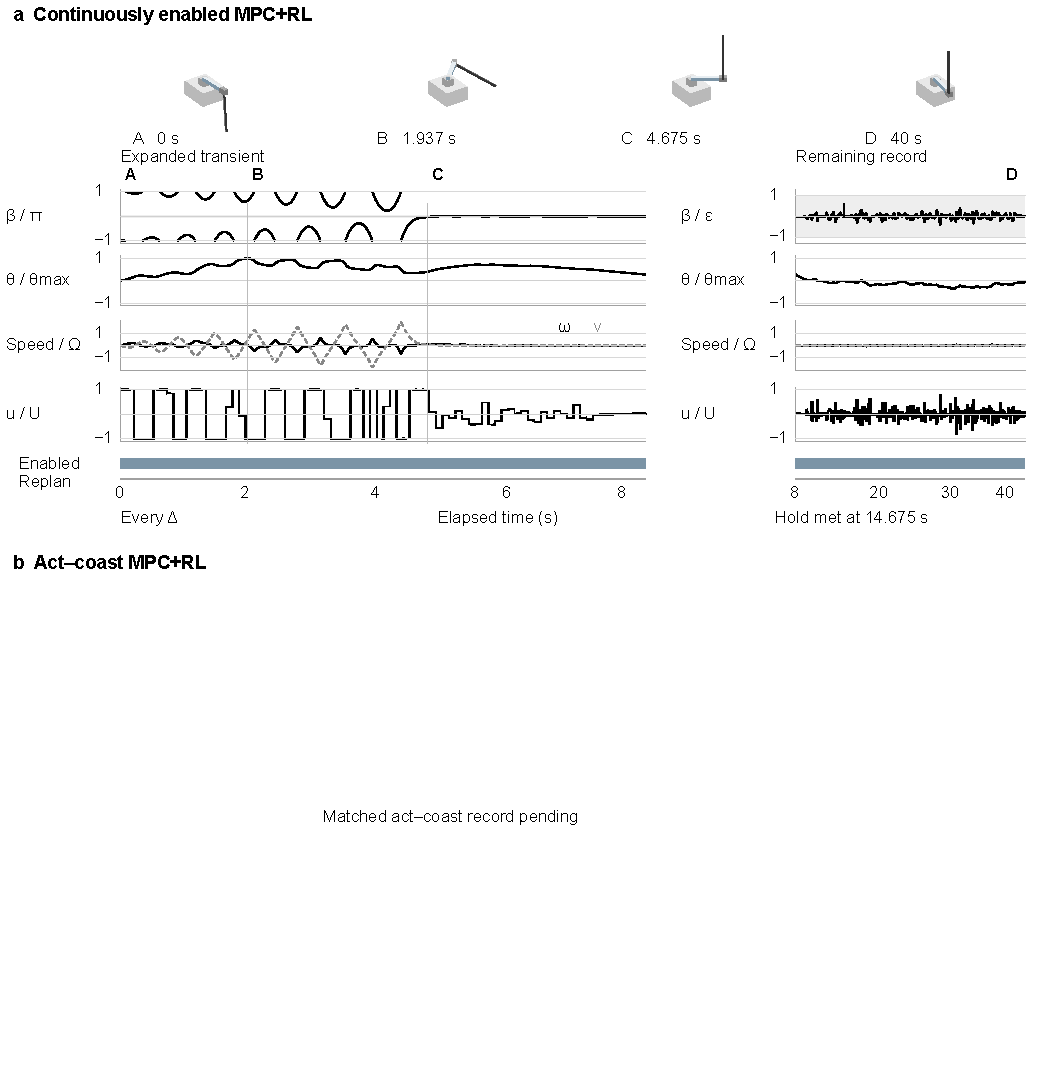
\includegraphics[width=\textwidth]{figures/session-record/figure-4-session-record.pdf}
\caption{Recorded motion and control activity.
(a) The fixed downward-neighborhood MPC+RL session. Adjacent linear views show the expanded initial segment and the complete remainder; no elapsed interval is omitted. Upright error $\beta=\operatorname{wrap}(\alpha-\pi)$ uses $\beta/\pi$ at left and $\beta/\varepsilon$ at right, where $\alpha$ is the pendulum angle from downward, wrapping selects $[-\pi,\pi)$, and $\varepsilon$ is the assessment tolerance. Curve breaks mark angular wrapping, not missing samples. Gray shading denotes this tolerance and the zero line denotes ideal upright orientation. Arm angle $\theta$ is divided by its prescribed bound $\theta_{\max}$; arm speed $\omega$ (black) and pendulum speed $\nu$ (gray dashed) share the downward small-motion frequency $\Omega$. Applied torque $u/U$, with cap $U>0$, is drawn as held commands. The blue rail denotes continuous enablement; torque magnitude does not determine mode. Feedback repeats every command interval $\Delta$. The short tick in the right error plot marks completion of the required holding duration.
Keyframes use one camera and recorded states: A is the initial condition, B the largest arm excursion before first upright-band entry, C that first entry, and D the final state. Their strip is not time-proportional; letters and timestamps identify the matching trace positions.
(b) The matched act--coast record is pending, so its configurations, curves, modes and events remain blank. These are simulated configurations, not hardware observations.}
\label{fig:session-record}
\end{figure*}


\subsection{Act--coast task--resource tradeoff}
\label{sec:results-tradeoff}
% Planned comparison links common task requirements to resource use.
Matched starts and costs $\rightarrow$ task satisfaction and violations $\rightarrow$ enabled fraction, decision rate, effort, and error.

Figure~\ref{fig:atlas} reserves the matched scenario comparison of task performance and resource use.

% Reserve the matched scenario comparison without implying measured results.
\begin{figure*}[t]
\centering
\fbox{%
\begin{minipage}[c][2.5in][c]{\dimexpr\textwidth-2\fboxsep-2\fboxrule\relax}
\centering
\textbf{Act--coast performance atlas}\par\medskip
Scenario columns with a declared pooled summary\par\medskip
Task and constraint status\par
Activation count \quad Enabled time \quad Online computation time\par
Replanning count as a separate diagnostic\par\medskip
Act--coast, bang--bang, event-triggered MPC,\par
maximum hands-off control, and mixed temporal resolution MPC\par\medskip
\textit{Matched comparison records pending}
\end{minipage}}
\caption{Placeholder for the aggregate act--coast performance comparison.
Scenario columns compare the proposed controller with bang--bang control, event-triggered MPC, maximum hands-off control, and mixed temporal resolution MPC under common dynamics, initial states, limits, holding criteria, and assessment duration. A task-success and constraint-status strip accompanies the resource rows so failed or shortened runs cannot appear as resource savings. Activation count $N_{\mathrm{on}}$ counts off-to-on mode transitions, including initial enablement when applicable. Enabled time $T_{\mathrm{on}}$ accumulates all enabled intervals, including enabled zero commands. Online computation time $C_{\mathrm{cmp}}$ sums non-overlapping controller timings, counting nested outer and inner optimization once; replanning count $n(T)$ separately counts feedback decisions over assessment duration $T$. The intended panels retain scenario-level distributions and trial denominators, with failed-run exposure identified separately and any pooled weighting declared. Computation comparisons require matched hardware and distinguish batch throughput from single-session latency. No comparison measurements are shown.}
\label{fig:atlas}
\end{figure*}


\subsection{Contribution of joint timing optimization}
\label{sec:results-timing}
% Planned ablations separate the contributions of the two outer timing decisions.
Joint timing versus fixed shut-off or fixed replanning $\rightarrow$ matched inner controller and budgets $\rightarrow$ timing contributions.

\subsection{Admissibility and operating limits}
\label{sec:results-admissibility}
% Planned boundary studies relate admissibility conditions to trajectory checks.
Declared domain and admissibility condition $\rightarrow$ limiting coast durations and fine replay $\rightarrow$ feasible timing pairs and violations.

\begin{thebibliography}{9}
\bibitem{heemels2012}
W. P. M. H. Heemels, K. H. Johansson, and P. Tabuada,
``An introduction to event-triggered and self-triggered control,''
in \emph{Proceedings of the 51st IEEE Conference on Decision and Control},
2012, pp. 3270--3285. \href{https://doi.org/10.1109/CDC.2012.6425820}{doi:10.1109/CDC.2012.6425820}.
\bibitem{astrom2000}
K. J. \AA str\"om and K. Furuta,
``Swinging up a pendulum by energy control,''
\emph{Automatica}, vol. 36, no. 2, 2000.
\href{https://doi.org/10.1016/S0005-1098(99)00140-5}{doi:10.1016/S0005-1098(99)00140-5}.
\bibitem{fujimoto2018}
S. Fujimoto, H. van Hoof, and D. Meger,
``Addressing function approximation error in actor-critic methods,''
in \emph{Proceedings of the 35th International Conference on Machine Learning},
vol. 80, 2018, pp. 1587--1596.
\href{https://proceedings.mlr.press/v80/fujimoto18a.html}{PMLR}.
\end{thebibliography}
\end{document}
